\باب{برقرار مقناطیسی میدان}
برقی میدان کا منبع برقی چارج ہے جس پر باب \حوالہ{باب_کولومب_قانون} میں تفصیلی غور کیا گیا۔مقناطیسی میدان کا منبع یا تو مقناطیس ہو سکتا ہے، یا وقت کے ساتھ بدلتا برقی میدان اور یا پھر برقی رو۔اس کتاب میں مقناطیس سے پیدا مقناطیسی میدان پر غور نہیں کیا جائے گا۔وقت کے ساتھ بدلتے برقی میدان سے پیدا مقناطیسی میدان پر ایک اور باب میں غور کیا جائے گا جبکہ اس باب میں برقی رو سے پیدا مقناطیسی میدان پر غور کیا جائے گا۔

\حصہ{بایوٹ-سیوارٹ کا قانون}
برقی رو اور اس سے پیدا مقناطیسی میدان کا تعلق \اصطلاح{بایوٹ-سیوارٹ}\فرہنگ{بایوٹ-سیوارٹ}\حاشیہب{Biot-Savart law}\فرہنگ{Biot-Savart law} کا قانون\حاشیہد{یہ قانون فرانس کے  بایوٹ اور سیوارٹ نے 1820 میں پیش کیا۔یہ دونوں ایمپیئر کے ساتھی تھے۔}
\begin{align}\label{مساوات_بایوٹ_سیوارٹ_تفرق_شکل}
\dif \kvec{H}=\frac{I \dif \kvec{L} \times \aR}{4 \pi R^2}
\end{align}
 بیان کرتا ہے جہاں سے مقناطیسی شدت \عددیء{\kvec{H}} کی اکائی ایمپیئر فی میٹر \عددیء{(\si{\ampere \per \meter})} حاصل ہوتی ہے۔آئیں اس قانون کا مطلب سمجھیں۔

یہ قانون باریک تار کے انتہائی چھوٹے حصے \عددیء{\dif \kvec{L}} جس میں \عددیء{I} برقی رو گزر رہا ہو سے  نقطہ \عددیء{P} پر پیدا سمتی برقی میدان \عددیء{\kvec{H}} دیتا ہے۔نقطہ \عددیء{P} باریک تار کے چھوٹی لمبائی سے \عددیء{\kvec{R}} فاصلے پر ہے۔باریک تار سے مراد ایسی ٹھوس نلکی نما موصل تار ہے جس کے رقبہ عمودی تراش کا رداس اتنا کم کر دیا جائے کہ یہ صفر کے قریب تر ہو۔\عددیء{\dif \kvec{L}} کی سمت برقی رو کی سمت میں ہے جبکہ \عددیء{I \dif \kvec{L}} منبع مقناطیسی میدان ہے۔

مقناطیسی شدت کی قیمت برقی رو ضرب باریک چھوٹی تار کی لمبائی ضرب \عددیء{\kvec{R}} اور \عددیء{\dif \kvec{L}} کے مابین زاویہ کے سائن کے برائے راست تناسب جبکہ ان کے مابین فاصلہ \عددیء{R} کے مربع کے بالعکس تناسب رکھتی ہے۔تناسبی مستقل \عددیء{\tfrac{1}{4\pi}} ہے۔

بایوٹ-سیوارٹ کے  قانون کا موازنہ کولومب کے قانون کے ساتھ کرنے کی غرض سے دونوں مساوات کو ایک ساتھ لکھتے ہیں۔
\begin{align*}
\dif \kvec{H}_2&=\frac{I_1 \dif \kvec{L}_1 \times \kvec{a}_{R21}}{4 \pi R_{21}^2}\\
\dif \kvec{E}_2&=\frac{\dif Q_1 \kvec{a}_{R21}}{4\pi \epsilon_0 R_{21}^2}
\end{align*}
ان مساوات میں زیر نوشت میں \عددیء{2} اس مقام کو ظاہر کرتی ہے جہاں میدان کی قیمت حاصل کی گئی ہے جبکہ زیر نوشت میں \عددیء{1} میدان کے منبع کے مقام کو ظاہر کرتی ہے۔دونوں میدان فاصلے کے مربع کا بالعکس تناسب رکھتے ہیں۔دونوں اقسام کے میدان کی شدت اور میدان کی منبع کا خطی تعلق ہے۔دونوں میں فرق میدان کی سمت کا ہے۔برقی میدان کی سمت منبع سے اس نقطہ کی جانب ہے جہاں میدان حاصل کیا جا رہے ہو۔مقناطیسی میدان کی سمت سمتی ضرب کے دائیں ہاتھ کے قانون سے حاصل ہوتی ہے۔

بایوٹ-سیوارٹ کے قانون کو مساوات \حوالہ{مساوات_بایوٹ_سیوارٹ_تفرق_شکل} کی شکل میں تجرباتی طور پر ثابت نہیں کیا جا سکتا چونکہ باریک تار کے چھوٹی لمبائی میں برقی رو تب گزرے گی جب یہ اس تک پہنچائی جائے۔جو تار اس تک برقی رو پہنچائے گا، وہ بھی مقناطیسی میدان پیدا کرے گا۔انہیں علیحدہ علیحدہ نہیں کیا جا سکتا۔یوں بایوٹ-سیوارٹ قانون کی تکمل شکل
\begin{align}\label{مساوات_بایوٹ_سیوارٹ_تکمل_شکل}
\kvec{H}=\oint \frac{I \dif \kvec{L} \times \aR}{4 \pi R^2}
\end{align}
ہی تجرباتی طور ثابت کی جا سکتی ہے۔

مساوات \حوالہ{مساوات_بایوٹ_سیوارٹ_تفرق_شکل} سے مساوات \حوالہ{مساوات_بایوٹ_سیوارٹ_تکمل_شکل} لکھی جا سکتی ہے۔البتہ مساوات \حوالہ{مساوات_بایوٹ_سیوارٹ_تکمل_شکل} میں تکمل کے اندر کوئی بھی ایسی اضافی تفاعل شامل کیا جا سکتا ہے جس کا بند تکمل صفر کے برابر ہو۔مقداری میدان کا ڈھلان ہر صورت بقائی میدان ہوتا ہے لہٰذا مساوات \حوالہ{مساوات_بایوٹ_سیوارٹ_تکمل_شکل} میں \عددیء{\nabla G} کے شمول سے اس کے جواب میں کوئی فرق نہیں پڑے گا۔\عددیء{G} کوئی بھی مقداری میدان ہو سکتا ہے۔اس حقیقت کا تذکرہ اس لئے کیا جا رہا ہے کہ اگر ہم ایک چھوٹے برقی رو گزارتے تار پر دوسرے  چھوٹے برقی رو گزارتے تار سے پیدا قوت دریافت کرنا چاہیں جہاں تجرباتی طور پر ان کا میدان قابل دریافت نہ ہو تب ہمیں احمقانہ جوابات ہی حاصل ہوں گے۔

بایوٹ-سیوارٹ کے قانون کو سطحی کثافت برقی رو \عددیء{\kvec{K}} یا کثافت برقی رو \عددیء{\kvec{J}} کی صورت میں بھی لکھا جا سکتا ہے جہاں
\begin{align}
I \dif \kvec{L}=\kvec{K} \dif S=\kvec{J} \dif v
\end{align}
لکھا جائے گا۔ یوں بایوٹ-سیوارٹ کے قانون کو
\begin{align}
\kvec{H}=\int_S \frac{\kvec{K} \times \aR \dif S}{4\pi R^2}
\end{align}
یا
\begin{align}
\kvec{H}=\int_h \frac{\kvec{J} \times \aR \dif h}{4\pi R^2}
\end{align}
لکھا جا سکتا ہے۔

\begin{figure}
\centering
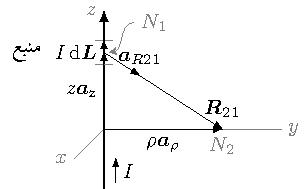
\includegraphics{figMagneticInfiniteStraightWiresField}
\caption{سیدھی لامحدود تار سے پیدا مقناطیسی میدان}
\label{شکل_مقناطیسی_سیدھی_لامحدود_تار_کا_میدان}
\end{figure}
آئیں برقی رو گزارتے سیدھی  لامحدود لمبائی کے تار سے پیدا مقناطیسی میدان بایوٹ-سیوارٹ کے قانون سے حاصل کریں۔شکل \حوالہ{شکل_مقناطیسی_سیدھی_لامحدود_تار_کا_میدان} میں صورت حال دکھائی گئی ہے۔اس تار کے دونوں سرے لامحدود فاصلے پر ہیں۔تار کے قریب نقطہ \عددیء{N} پر مقناطیسی میدان کا بیشتر حصہ تار کے اس حصے کی وجہ سے ہو گا جو \عددیء{N} کے قریب ہو۔یوں لامحدود فاصلے پر تار کے سروں تک برقی رو پہنچانے  والے تار کا نقطہ \عددیء{N} پر اثر کو نظرانداز کرتے ہوئے آگے بڑھتے ہیں۔ 

نقطہ \عددیء{N_1} پر تار کے چھوٹے حصے \عددیء{\dif \kvec{L}} کو منبع مقناطیسی میدان تصور کرتے ہوئے مساوات \حوالہ{مساوات_بایوٹ_سیوارٹ_تفرق_شکل} کی مدد سے نقطہ \عددیء{N_2} پر مقناطیسی میدان لکھی جا سکتی ہے۔چونکہ 
\begin{align*}
\kvec{R}_{21}=\rho \arho-z \az
\end{align*}
کے برابر ہے لہٰذا
\begin{align*}
R_{21}&=\abs{\kvec{R}_{21}}=\sqrt{\rho^2+z^2}\\
\aR&=\frac{\kvec{R}_{21}}{\abs{\kvec{R}_{21}}}=\frac{\rho \arho-z \az}{\sqrt{\rho^2+z^2}}
\end{align*}
لکھے جا سکتے ہیں۔نلکی محدد میں چھوٹی لمبائی
\begin{align*}
\dif \kvec{L}=\dif \rho \arho+\rho \dif \phi \aphi+\dif z \az
\end{align*}
لکھی جاتی ہے۔چونکہ یہاں \عددیء{\dif \rho=0} اور \عددیء{\dif \phi=0} ہیں لہٰذا \عددیء{\dif \kvec{L}=\dif z \az} لکھتے ہوئے  مساوات \حوالہ{مساوات_بایوٹ_سیوارٹ_تفرق_شکل} کو
\begin{align*}
\dif \kvec{H}_2=\frac{I \dif z \az \times (\rho \arho -z\az)}{4 \pi (\rho^2+z^2)^{\frac{3}{2}}}
\end{align*}
لکھا جا سکتا ہے۔پورے تار کا مقناطیسی میدان اس مساوات کے تکمل سے حاصل ہو گا جہاں تکمل\عددیء{-\infty} تا \عددیء{+\infty} حاصل کیا جائے گا۔اس طرح
\begin{align*}
\kvec{H}_2&=\int_{-\infty}^{\infty}\frac{I \dif z \az \times (\rho \arho -z\az)}{4 \pi (\rho^2+z^2)^{\frac{3}{2}}}\\
&=\frac{I \rho}{4\pi}\int_{-\infty}^{\infty} \frac{\aphi \dif z }{(\rho^2+z^2)^{\frac{3}{2}}}
\end{align*}    
لکھا جا سکتا ہے جہاں صفحہ \حوالہصفحہ{مساوات_سمتیات_نلکی_اکائی_سمتیات_کا_سمتی_ضرب} پر مساوات \حوالہ{مساوات_سمتیات_نلکی_اکائی_سمتیات_کا_سمتی_ضرب} کی مدد سے \عددیء{\az \times \arho=\aphi} جبکہ مساوات \حوالہ{مساوات_سمتیات_نلکی_اکائی_سمتیات_کا_سمتی_ضرب_ب} کی مدد سے \عددیء{\az \times \az=0} لکھے گئے ہیں۔

مندرجہ بالا مساوات میں تکمل کے اندر \عددیء{\aphi} پر نظر رکھنا ہو گا۔اگرچہ \عددیء{\aphi} اکائی سمتیہ ہے لہٰذا اس کی لمبائی تبدیل نہیں ہو سکتی البتہ یہ دیکھنا ضروری ہے کہ آیا تکمل کا متغیرہ یعنی \عددیء{z} تبدیل کرنے سے \عددیء{\aphi} کی سمت تو تبدیل نہیں ہوتی۔صفحہ \حوالہصفحہ{مساوات_سمتیہ_اکائی_زاویہ_کارتیسی_میں} پر مساوات \حوالہ{مساوات_سمتیہ_اکائی_زاویہ_کارتیسی_میں} کے تحت
\begin{align*}
\aphi&=-\frac{y}{\sqrt{x^2+y^2}} \ax+\frac{x}{\sqrt{x^2+y^2}} \ay
\end{align*}
لکھا جا سکتا ہے۔آپ دیکھ سکتے ہیں کہ \عددیء{z} تبدیل کرنے سے \عددیء{\aphi} پر کوئی اثر نہیں پڑتا لہٰذا \عددیء{\aphi} کو تکمل کے باہر منتقل کیا جا سکتا ہے۔یوں
\begin{gather}
\begin{aligned}\label{مساوات_مقناطیسی_سیدھی_لامحدود_تار_کا_میدان}
\kvec{H}_2&=\frac{I \rho\aphi}{4\pi}\int_{-\infty}^{\infty} \frac{\dif z }{(\rho^2+z^2)^{\frac{3}{2}}}\\
&=\eval{\frac{I \rho \aphi}{4\pi} \frac{z}{\rho^2 \sqrt{\rho^2+z^2}}}_{-\infty}^{+\infty}
\end{aligned}
\end{gather}    
سے
\begin{align}
\kvec{H}_2=\frac{I}{2\pi \rho} \aphi
\end{align}
حاصل ہوتا ہے۔شکل \حوالہ{شکل_مقناطیسی_سیدھے_تار_کا_میدان_دائرے} میں برقی رو صفحہ سے باہر نکل رہی ہے جبکہ گول دائرے مقناطیسی میدان کو ظاہر کرتے ہیں۔اگر تار کو دائیں ہاتھ سے یوں پکڑا جائے کہ انگوٹھا برقی رو کی سمت میں ہو تب اس ہاتھ کی انگلیاں تار کے گرد مقناطیسی میدان کی سمت میں لپٹی ہوں گی۔آپ دیکھ سکتے ہیں کہ یہ مقناطیسی میدان نا نو \عددیء{z} اور نا ہی زاویہ \عددیء{\phi} کے ساتھ تبدیل ہوتا ہے۔اس کی قیمت صرف تار سے فاصلے پر منحصر ہے۔
\begin{figure}
\centering
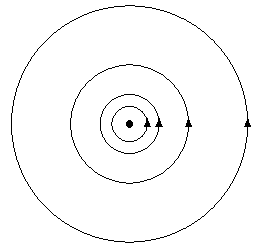
\includegraphics{figMagneticInfiniteStraightWiresStreamlines}
\caption{سیدھی لمبی تار کا مقناطیسی میدان تار کے گرد دائرے بناتا ہے۔برقی رو صفحے سے باہر نکل رہی ہے۔}
\label{شکل_مقناطیسی_سیدھے_تار_کا_میدان_دائرے}
\end{figure}
%
\begin{figure}
\centering
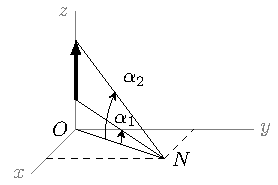
\includegraphics{figMagneticStraightWiresField}
\caption{سیدھی  محدود لمبائی کے تار کی مقناطیسی شدت۔}
\label{شکل_مقناطیسی_سیدھے_محدود_تار_کا_میدان}
\end{figure}

اگر شکل \حوالہ{شکل_مقناطیسی_سیدھی_لامحدود_تار_کا_میدان} میں تار لامحدود نہ ہو تب مساوات \حوالہ{شکل_مقناطیسی_سیدھے_محدود_تار_کا_میدان} میں تکمل کے محدود حدود پر کرنے سے مقناطیسی میدان کی شدت
\begin{align}\label{مساوات_مقناطیسی_محدود_تار_کی_مقناطیس}
\kvec{H}=\frac{I}{4\pi \rho} \left(\sin \alpha_2-\sin \alpha_1 \right) \aphi
\end{align}
حاصل ہوتی ہے جہاں شکل \حوالہ{شکل_مقناطیسی_سیدھے_محدود_تار_کا_میدان} میں \عددیء{\alpha_1} اور \عددیء{\alpha_2} کی نشاندہی کی گئی ہے۔تار کا نچلا سرا \عددیء{xy} سطح یعنی \عددیء{z=0} سطح سے نیچے ہونے کی صورت میں \عددیء{\alpha_1} کی قیمت منفی ہو گی۔یہی کچھ تار کے دوسرے سرے اور \عددیء{\alpha_2} کے لئے بھی درست ہے۔

\حصہ{ایمپیئر کا دوری قانون}
کولومب کے قانون کی مدد سے مختلف طرز پر پائے جانے والے چارج کے برقی میدان حاصل کرنے کے بعد ہم نے گاؤس کا قانون اخذ کیا جس سے ہماری زندگی نہایت آسان ہو گئی۔گاؤس کے قانون کی مدد سے متشاکل چارج سے پیدا برقی میدان انتہائی آسانی سے حاصل ہوتا ہے۔متشاکل برقی رو کے مقناطیسی میدان حاصل کرنے کا بھی اتنا ہی آسان طریقہ موجود ہے جسے \اصطلاح{ایمپیئر کا دوری قانون}\فرہنگ{ایمپیئر کا دوری قانون}\حاشیہب{Ampere's circuital law}\فرہنگ{Ampere's circuital law} کہتے ہیں۔اس قانون کو بایوٹ-سیوارٹ کے قانون سے آگے جا کر حاصل کیا گیا ہے۔فی الحال ہم اس قانون کو استعمال کرنا سیکھتے ہیں۔اس قانون کے استعمال کے وقت مسئلے پر غور کرتے ہوئے بغیر حساب و کتاب کے فیصلہ کیا جاتا ہے کہ مقناطیسی میدان کے کون کون سے اجزاء موجود نہیں ہونے چاہئے۔یہ فیصلہ برقی رو کے راستے کو دیکھ کر کیا جاتا ہے۔

ایمپیئر کا دوری قانون کہتا ہے کہ یک سمتی برقی رو کے گرد کسی بھی راہ \عددیء{\kvec{H}} کا لکیری بند تکمل گھیرے برقی رو کے برابر ہو گا یعنی
\begin{align}\label{مساوات_مقناطیسی_ایمپیئر_کا_دوری_قانون}
\oint \kvec{H} \cdot \dif \kvec{L}=I
\end{align}

لکیری بند تکمل کی سمت میں برقی رو کے گرد  دائیں ہاتھ کی انگلیاں گھمانے سے اسی ہاتھ کا انگوٹھا مثبت برقی رو کی سمت دے گا۔ایسا کرتے وقت انگوٹھے کو باقی چار انگلیوں کے عمودی رکھا جاتا ہے۔

کسی بھی راہ \عددیء{\kvec{H}} کے لکیری تکمل سے مراد اس راہ  کو انتہائی چھوٹے چھوٹے ٹکڑوں \عددیء{\dif \kvec{L}} میں تقسیم کر کے ہر ٹکڑے پر \عددیء{\kvec{H}} کی قیمت استعمال کرتے ہوئے \عددی{\kvec{H} \cdot \dif \kvec{L}} حاصل کر کے تمام \عددی{\kvec{H} \cdot \dif \kvec{L}} کا مجموعہ حاصل کرنا ہے۔مقناطیسی شدت \عددیء{\kvec{H}} کی قیمت مختلف مقامات پر عموماً مختلف ہو گی۔یوں کسی ایک نقطے پر \عددی{\kvec{H} \cdot \dif \kvec{L}} کی قیمت کسی دوسرے نقطے کے \عددی{\kvec{H} \cdot \dif \kvec{L}} سے مختلف ہو گی۔ایمپیئر کا دوری قانون کہتا ہے کہ اگرچہ یک سمتی برقی رو کے گرد دو مختلف بند راہوں پر جگہ جگہ \عددی{\kvec{H} \cdot \dif \kvec{L}} کی قیمتیں مختلف ہوں گی لیکن دونوں راہ پر ان کا مجموعہ عین برقی رو کے برابر ہو گا۔

کسی بھی سطح کا محیط، بند راہ ہوتی ہے۔اسی طرح کوئی بھی بند راہ، لامحدود سطحوں کا محیط ہوتا ہے۔یوں بند راہ کا گھیرا ہوا برقی رو ان تمام سطحوں کو چھیرتا ہوا گزرے گا جن کا محیط یہ بند راہ ہو۔

گاؤس کے قانون کا استعمال تب ممکن ہوتا ہے جب بند سطح میں کل برقی چارج معلوم ہو۔ایمپیئر کا دوری قانون اس صورت استعمال کیا جا سکتا ہے جب  بند راہ میں گھیرا کل یک سمتی برقی رو معلوم ہو۔   

آئیں شکل \حوالہ{شکل_مقناطیسی_سیدھی_لامحدود_تار_کا_میدان} میں دکھائے گئے  برقی رو گزارتے سیدھی لامحدود لمبائی کے تار کی مقناطیسی شدت ایمپیئر کے دوری قانون یعنی مساوات \حوالہ{مساوات_مقناطیسی_ایمپیئر_کا_دوری_قانون} کی مدد سے دوبارہ حاصل کریں۔اس مساوات کو استعمال کرتے ہوئے  برقی رو کے گرد راہ یوں چنی جاتے ہے کہ اس پر \عددیء{\kvec{H}} اور \عددیء{\dif \kvec{L}} یا تو آپس میں عمودی ہوں اور یا \عددیء{\kvec{H}} کی قیمت قطعی اور اس کی سمت \عددیء{\dif \kvec{L}} کے متوازی ہو۔پہلی صورت میں دونوں متغیرات کے مابین نوے درجے کا زاویہ  ہے اور \عددیء{\cos 90\degree=0} ہوتا ہے لہٰذا \عددیء{\kvec{H} \cdot \dif \kvec{L}} صفر کے برابر ہو گا اور یوں راہ کے اس حصے پر تکمل صفر کے برابر ہو گا۔ دوسری صورت میں متغیرات کے مابین صفر درجے کا زاویہ ہے اور \عددیء{\cos 0 \degree=1} ہوتا ہے لہٰذا \عددیء{\kvec{H} \cdot \dif \kvec{L}}  کو \عددیء{H \dif L} لکھا جا سکتا ہے اور ساتھ ہی ساتھ مقناطیسی شدت کی قیمت قطعی ہونے کی وجہ سے \عددیء{H} کو تکمل کے باہر لے جایا جا سکتا ہے۔یوں راہ کے اس راستے پر تکمل کی قیمت \عددیء{H L} کے برابر ہو گی جہاں \عددیء{L} راہ کے اس حصے کی لمبائی ہے۔

تار کے گرد اور اس کے ساتھ ساتھ حرکت کرنے سے واضح ہوتا ہے کہ مسئلے کی نوعیت نا تو تار کے گرد زاویہ \عددیء{\phi} پر اور نا ہی محدد \عددیء{z} پر منحصر ہے۔تار سے دور یا اس کے قریب ہونے سے ہی مسئلے کی نوعیت میں تبدیلی آتی ہے۔یوں صاف ظاہر ہے کہ مقناطیسی شدت صرف \عددیء{\rho} پر منحصر ہو سکتی ہے۔اسی طرح بایوٹ-سیوارٹ کے قانون کو مد نظر رکھتے ہوئے ہم دیکھ سکتے ہیں کہ مقناطیسی شدت \عددیء{\aphi} سمت رکھتی ہے یعنی اس کا صرف \عددیء{H_{\phi}} جزو پایا جائے گا۔یوں اگر \عددیء{\rho} تبدیل کئے بغیر تار کے گرد چلا جائے تو ہم یقین رکھ سکتے ہیں کہ \عددیء{\kvec{H}} کی حتمی قیمت \عددیء{H_{\phi}} تبدیل نہیں ہو گی۔ساتھ ہی ساتھ اس راہ پر کسی بھی نقطے پر  \عددیء{\dif \kvec{L}=\rho \dif \phi \aphi} اور \عددیء{H_{\phi} \aphi} آپس میں متوازی ہوں گے لہٰذا ایمپیئر کے دوری قانون سے
\begin{align*}
\oint \kvec{H} \cdot \dif \kvec{L}=\int_0^{2\pi} H_{\phi} \rho \dif \phi=H_{\phi} \rho \int_0^{2\pi} \dif \phi=H_{\phi} 2\pi \rho=I
\end{align*}
یا
\begin{align*}
H_{\phi}=\frac{I}{2\pi \rho}
\end{align*}
حاصل ہوتا ہے جو ہم پہلے بھی حاصل کر چکے ہیں۔

ایمپیئر کے دوری قانون  کے استعمال کی دوسری مثال کی خاطر ہم محوری تار لیتے ہوئے آگے بڑھتے ہیں۔فرض کریں کہ \عددیء{z} محدد پر پڑی  ایسی لامحدود لمبائی کے ہم محوری  تار کے اندرونی حصے میں \عددیء{I} اور اس کے بیرونی سطح میں \عددیء{-I} برقی رو گزر رہی ہے۔اندرونی موصل موٹی ساخت کے تار کو نہایت پتلی تاروں کا مجموعہ تصور کیا جا سکتا ہے۔آئیں ان پتلی تاروں سے نقطہ \عددیء{N} پر پیدا مقناطیسی شدت پر غور کریں۔پچھلی مثال سے یہ واضح ہے کہ ایسی کسی بھی پتلی تار کی مقناطیسی شدت میں \عددیء{H_z} جزو نہیں پایا جاتا۔\عددیء{(\rho_1,\phi_1)}پر ایسی پتلی تار سے پیدا مقناطیسی شدت کے نقطہ \عددیء{N} پر  \عددیء{H_{\rho}} اور \عددیء{H_{\phi}} اجزاء ہوں گے۔اسی طرح \عددیء{(\rho_1,-\phi_1)} پر پتلی تار سے پیدا مقناطیسی شدت کے بھی ایسے اجزاء ہوں گے۔ان دونوں پتلی تاروں کے \عددیء{H_{\rho}} اجزاء آپس میں الٹ سمت میں ہوں گے لہٰذا یہ ایک دونوں کو ختم کرتے ہیں ۔چونکہ \عددیء{N} کے دونوں جانب کے پتلے تار \عددیء{N} پر آپس کے رداسی مقناطیسی اجزاء ختم کرتے ہیں لہٰذا \عددیء{N} پر صرف \عددیء{H_{\phi}} پایا جائے گا۔شکل میں اس حقیقت کی وضاحت کی گئی ہے۔

اندرونی ٹھوس موصل تار کے گرد ایسا گول دائرہ لیتے ہیں جس کا رداس \عددیء{\rho} اندرونی تار کے رداس \عددیء{a} سے زیادہ مگر بیرونی تار کے اندرونی رداس \عددیء{b} سے کم ہو۔اس راہ پر ہم ایمپیئر کے دوری قانون کی مدد سے
\begin{align*}
H_{\phi}=\frac{I}{2\pi \rho} \quad \quad (a < \rho <b)
\end{align*}
لکھ سکتے ہیں۔

اگر \عددیء{\rho} کو اندرونی ٹھوس موصل تار کے رداس \عددیء{a} سے کم رکھا جائے تب یہ راہ
\begin{align*}
I_{\textrm{گھیرا}}=\frac{\rho^2}{a^2} I
\end{align*}
برقی رو کو گھیرے گا لہٰذا ایمپیئر کا دوری قانون، اندرونی ٹھوس تار کے اندر
\begin{align*}
H_{\phi}=\frac{\rho I}{2\pi a^2} \quad \quad (\rho < a)
\end{align*}
مقناطیسی شدت دے گا۔اسی طرح اگر \عددیء{} کو بیرونی تار کے بیرونی رداس \عددیء{c} سے زیادہ رکھا جائے تب یہ راہ کل \عددیء{I-I=0} برقی رو کو گھیرے گا لہٰذا 
\begin{align*}
H_{\phi} =0 \quad \quad (\rho >c)
\end{align*}
ہو گا۔آخر میں اس صورت کو بھی دیکھتے ہیں جب \عددیء{\rho} بیرونی تار کے اندر پایا جائے۔ایسی صورت میں یہ راہ
\begin{align*}
I_{\textrm{گھیرا}}=I-\left(\frac{\rho^2-b^2}{c^2-b^2}\right) I=\left(\frac{c^2-\rho^2}{c^2-b^2}\right)I
\end{align*}
برقی رو گھیرے گی لہٰذا بیرونی تار کے اندر
\begin{align*}
H_{\phi}=\frac{I}{2\pi \rho} \left(\frac{c^2-\rho^2}{c^2-b^2} \right) \quad \quad (b<\rho<c)
\end{align*}
ہو گا۔ 
